% Options for packages loaded elsewhere
\PassOptionsToPackage{unicode}{hyperref}
\PassOptionsToPackage{hyphens}{url}
%
\documentclass[
  ignorenonframetext,
]{beamer}
\usepackage{pgfpages}
\setbeamertemplate{caption}[numbered]
\setbeamertemplate{caption label separator}{: }
\setbeamercolor{caption name}{fg=normal text.fg}
\beamertemplatenavigationsymbolsempty
% Prevent slide breaks in the middle of a paragraph
\widowpenalties 1 10000
\raggedbottom
\setbeamertemplate{part page}{
  \centering
  \begin{beamercolorbox}[sep=16pt,center]{part title}
    \usebeamerfont{part title}\insertpart\par
  \end{beamercolorbox}
}
\setbeamertemplate{section page}{
  \centering
  \begin{beamercolorbox}[sep=12pt,center]{part title}
    \usebeamerfont{section title}\insertsection\par
  \end{beamercolorbox}
}
\setbeamertemplate{subsection page}{
  \centering
  \begin{beamercolorbox}[sep=8pt,center]{part title}
    \usebeamerfont{subsection title}\insertsubsection\par
  \end{beamercolorbox}
}
\AtBeginPart{
  \frame{\partpage}
}
\AtBeginSection{
  \ifbibliography
  \else
    \frame{\sectionpage}
  \fi
}
\AtBeginSubsection{
  \frame{\subsectionpage}
}
\usepackage{amsmath,amssymb}
\usepackage{iftex}
\ifPDFTeX
  \usepackage[T1]{fontenc}
  \usepackage[utf8]{inputenc}
  \usepackage{textcomp} % provide euro and other symbols
\else % if luatex or xetex
  \usepackage{unicode-math} % this also loads fontspec
  \defaultfontfeatures{Scale=MatchLowercase}
  \defaultfontfeatures[\rmfamily]{Ligatures=TeX,Scale=1}
\fi
\usepackage{lmodern}
\ifPDFTeX\else
  % xetex/luatex font selection
\fi
% Use upquote if available, for straight quotes in verbatim environments
\IfFileExists{upquote.sty}{\usepackage{upquote}}{}
\IfFileExists{microtype.sty}{% use microtype if available
  \usepackage[]{microtype}
  \UseMicrotypeSet[protrusion]{basicmath} % disable protrusion for tt fonts
}{}
\makeatletter
\@ifundefined{KOMAClassName}{% if non-KOMA class
  \IfFileExists{parskip.sty}{%
    \usepackage{parskip}
  }{% else
    \setlength{\parindent}{0pt}
    \setlength{\parskip}{6pt plus 2pt minus 1pt}}
}{% if KOMA class
  \KOMAoptions{parskip=half}}
\makeatother
\usepackage{xcolor}
\newif\ifbibliography
\usepackage{color}
\usepackage{fancyvrb}
\newcommand{\VerbBar}{|}
\newcommand{\VERB}{\Verb[commandchars=\\\{\}]}
\DefineVerbatimEnvironment{Highlighting}{Verbatim}{commandchars=\\\{\}}
% Add ',fontsize=\small' for more characters per line
\usepackage{framed}
\definecolor{shadecolor}{RGB}{248,248,248}
\newenvironment{Shaded}{\begin{snugshade}}{\end{snugshade}}
\newcommand{\AlertTok}[1]{\textcolor[rgb]{0.94,0.16,0.16}{#1}}
\newcommand{\AnnotationTok}[1]{\textcolor[rgb]{0.56,0.35,0.01}{\textbf{\textit{#1}}}}
\newcommand{\AttributeTok}[1]{\textcolor[rgb]{0.13,0.29,0.53}{#1}}
\newcommand{\BaseNTok}[1]{\textcolor[rgb]{0.00,0.00,0.81}{#1}}
\newcommand{\BuiltInTok}[1]{#1}
\newcommand{\CharTok}[1]{\textcolor[rgb]{0.31,0.60,0.02}{#1}}
\newcommand{\CommentTok}[1]{\textcolor[rgb]{0.56,0.35,0.01}{\textit{#1}}}
\newcommand{\CommentVarTok}[1]{\textcolor[rgb]{0.56,0.35,0.01}{\textbf{\textit{#1}}}}
\newcommand{\ConstantTok}[1]{\textcolor[rgb]{0.56,0.35,0.01}{#1}}
\newcommand{\ControlFlowTok}[1]{\textcolor[rgb]{0.13,0.29,0.53}{\textbf{#1}}}
\newcommand{\DataTypeTok}[1]{\textcolor[rgb]{0.13,0.29,0.53}{#1}}
\newcommand{\DecValTok}[1]{\textcolor[rgb]{0.00,0.00,0.81}{#1}}
\newcommand{\DocumentationTok}[1]{\textcolor[rgb]{0.56,0.35,0.01}{\textbf{\textit{#1}}}}
\newcommand{\ErrorTok}[1]{\textcolor[rgb]{0.64,0.00,0.00}{\textbf{#1}}}
\newcommand{\ExtensionTok}[1]{#1}
\newcommand{\FloatTok}[1]{\textcolor[rgb]{0.00,0.00,0.81}{#1}}
\newcommand{\FunctionTok}[1]{\textcolor[rgb]{0.13,0.29,0.53}{\textbf{#1}}}
\newcommand{\ImportTok}[1]{#1}
\newcommand{\InformationTok}[1]{\textcolor[rgb]{0.56,0.35,0.01}{\textbf{\textit{#1}}}}
\newcommand{\KeywordTok}[1]{\textcolor[rgb]{0.13,0.29,0.53}{\textbf{#1}}}
\newcommand{\NormalTok}[1]{#1}
\newcommand{\OperatorTok}[1]{\textcolor[rgb]{0.81,0.36,0.00}{\textbf{#1}}}
\newcommand{\OtherTok}[1]{\textcolor[rgb]{0.56,0.35,0.01}{#1}}
\newcommand{\PreprocessorTok}[1]{\textcolor[rgb]{0.56,0.35,0.01}{\textit{#1}}}
\newcommand{\RegionMarkerTok}[1]{#1}
\newcommand{\SpecialCharTok}[1]{\textcolor[rgb]{0.81,0.36,0.00}{\textbf{#1}}}
\newcommand{\SpecialStringTok}[1]{\textcolor[rgb]{0.31,0.60,0.02}{#1}}
\newcommand{\StringTok}[1]{\textcolor[rgb]{0.31,0.60,0.02}{#1}}
\newcommand{\VariableTok}[1]{\textcolor[rgb]{0.00,0.00,0.00}{#1}}
\newcommand{\VerbatimStringTok}[1]{\textcolor[rgb]{0.31,0.60,0.02}{#1}}
\newcommand{\WarningTok}[1]{\textcolor[rgb]{0.56,0.35,0.01}{\textbf{\textit{#1}}}}
\usepackage{longtable,booktabs,array}
\usepackage{calc} % for calculating minipage widths
\usepackage{caption}
% Make caption package work with longtable
\makeatletter
\def\fnum@table{\tablename~\thetable}
\makeatother
\usepackage{graphicx}
\makeatletter
\def\maxwidth{\ifdim\Gin@nat@width>\linewidth\linewidth\else\Gin@nat@width\fi}
\def\maxheight{\ifdim\Gin@nat@height>\textheight\textheight\else\Gin@nat@height\fi}
\makeatother
% Scale images if necessary, so that they will not overflow the page
% margins by default, and it is still possible to overwrite the defaults
% using explicit options in \includegraphics[width, height, ...]{}
\setkeys{Gin}{width=\maxwidth,height=\maxheight,keepaspectratio}
% Set default figure placement to htbp
\makeatletter
\def\fps@figure{htbp}
\makeatother
\setlength{\emergencystretch}{3em} % prevent overfull lines
\providecommand{\tightlist}{%
  \setlength{\itemsep}{0pt}\setlength{\parskip}{0pt}}
\setcounter{secnumdepth}{-\maxdimen} % remove section numbering
\ifLuaTeX
  \usepackage{selnolig}  % disable illegal ligatures
\fi
\IfFileExists{bookmark.sty}{\usepackage{bookmark}}{\usepackage{hyperref}}
\IfFileExists{xurl.sty}{\usepackage{xurl}}{} % add URL line breaks if available
\urlstyle{same}
\hypersetup{
  pdftitle={TMA4315 Generalized linear models},
  pdfauthor={Mette Langaas, Department of Mathematical Sciences, NTNU - with contributions from Øyvind Bakke, Thea Bjørnland and Ingeborg Hem},
  hidelinks,
  pdfcreator={LaTeX via pandoc}}

\title{TMA4315 Generalized linear models}
\subtitle{Module 3: BINARY REGRESSION}
\author{Mette Langaas, Department of Mathematical Sciences, NTNU - with
contributions from Øyvind Bakke, Thea Bjørnland and Ingeborg Hem}
\date{}

\begin{document}
\frame{\titlepage}

\begin{frame}{Overview}
\protect\hypertarget{overview}{}
\begin{block}{Learning material}
\protect\hypertarget{learning-material}{}
\begin{itemize}
\tightlist
\item
  Textbook: Fahrmeir et al (2013): Chapter 2.3, 5.1, B4.1-3
\item
  \href{https://www.math.ntnu.no/emner/TMA4315/2018h/TMA4315M3H20180913.pdf}{Classnotes
  13.09.2018}
\item
  \href{https://www.math.ntnu.no/emner/TMA4315/2018h/TMA4315M3H20180920.pdf}{Classnotes
  20.09.2018}
\end{itemize}
\end{block}
\end{frame}

\begin{frame}
\begin{block}{Topics}
\protect\hypertarget{topics}{}
\begin{block}{\protect\hyperlink{firstweek}{First week}}
\protect\hypertarget{first-week}{}
\begin{itemize}
\tightlist
\item
  aim of binary regression
\item
  how to model a binary response
\item
  three ingredients of a GLM model
\item
  the logit model: logistic regression
\item
  interpreting the logit model - with odds
\item
  grouped vs.~individual data
\item
  parameter estimation with maximum likelihood

  \begin{itemize}
  \tightlist
  \item
    likelihood, log-likelihood,
  \item
    score function
  \end{itemize}
\end{itemize}
\end{block}
\end{block}
\end{frame}

\begin{frame}[fragile]
\begin{block}{\protect\hyperlink{secondweek}{Second week}}
\protect\hypertarget{second-week}{}
\begin{itemize}
\tightlist
\item
  Parameter estimation

  \begin{itemize}
  \tightlist
  \item
    score function- and mean and covariance thereof,
  \item
    observed and expected information matrix
  \end{itemize}
\item
  comparison with the normal distribution - score function and Fisher
  information
\item
  exponential family and canonical link
\item
  iterative calculation of ML estimator (Newton-Raphson and Fisher
  scoring) - and in R with \texttt{optim}
\item
  asymptotic properties of ML estimators - how to use in inference?
\item
  statistical inference

  \begin{itemize}
  \tightlist
  \item
    confidence intervals
  \item
    hypothesis testing: Wald, and likelihood ratio
  \end{itemize}
\item
  deviance: definition, analysis of deviance, deviance residuals
\item
  model fit and model choice
\item
  overdispersion and estimating overdispersion parameter
\item
  sampling stragegy: cohort, but also case-control data good for logit
  model
\end{itemize}
\end{block}
\end{frame}

\begin{frame}{Aim of binary regression}
\protect\hypertarget{aim-of-binary-regression}{}
\begin{block}{Two aims}
\protect\hypertarget{two-aims}{}
\begin{enumerate}
\tightlist
\item
  Construct a model to help understand the relationship between a
  ``success probability'' and one or several explanatory variables. The
  response measurements are binary (present/absent, true/false,
  healthy/diseased).
\item
  Use the model for estimation and prediction of success probabilites.
\end{enumerate}

Two running examples: mortality of beetles and probability of
respiratory infant disease.
\end{block}
\end{frame}

\begin{frame}
\begin{block}{Example: Dose response of beetles}
\protect\hypertarget{example-dose-response-of-beetles}{}
A total of 481 beetles were exposed to 8 different concentration of
CS\(_2\) (data on log10-dose).

For each beetle is was recorded if the beetle was alive or killed at the
given concentration.

Data for beetle \(i\): \(Y_i=0\) if beetle \(i\) was alive and \(Y_i=1\)
if it was killed, and \(x_i\) is then the log10-dose beetle \(i\) was
given.
\end{block}
\end{frame}

\begin{frame}[fragile]
The table below shows the 8 values of the log10-dose against the number
of beetles alive and killed. The plot shows log10-dose on the horizontal
axis and fraction of beetles killed (killed/total) for each log10-dose.

\begin{Shaded}
\begin{Highlighting}[]
\FunctionTok{library}\NormalTok{(investr)}
\CommentTok{\# from aggregated to individual data (because these data were aggregated)}
\NormalTok{ldose}\OtherTok{=}\FunctionTok{rep}\NormalTok{(}\FunctionTok{round}\NormalTok{(beetle}\SpecialCharTok{$}\NormalTok{ldose, }\DecValTok{2}\NormalTok{), beetle}\SpecialCharTok{$}\NormalTok{n)}
\NormalTok{y}\OtherTok{=}\ConstantTok{NULL}\NormalTok{; }\ControlFlowTok{for}\NormalTok{ (i }\ControlFlowTok{in} \DecValTok{1}\SpecialCharTok{:}\DecValTok{8}\NormalTok{) y}\OtherTok{=}\FunctionTok{c}\NormalTok{(y,}\FunctionTok{rep}\NormalTok{(}\DecValTok{0}\NormalTok{,beetle}\SpecialCharTok{$}\NormalTok{n[i]}\SpecialCharTok{{-}}\NormalTok{beetle}\SpecialCharTok{$}\NormalTok{y[i]),}\FunctionTok{rep}\NormalTok{(}\DecValTok{1}\NormalTok{,beetle}\SpecialCharTok{$}\NormalTok{y[i]))}
\NormalTok{beetleds}\OtherTok{=}\FunctionTok{data.frame}\NormalTok{(}\StringTok{"killed"}\OtherTok{=}\NormalTok{y,}\StringTok{"ldose"}\OtherTok{=}\NormalTok{ldose)}
\NormalTok{knitr}\SpecialCharTok{::}\FunctionTok{kable}\NormalTok{(}\FunctionTok{table}\NormalTok{(beetleds), }\AttributeTok{digits =} \DecValTok{2}\NormalTok{)}
\end{Highlighting}
\end{Shaded}

\begin{longtable}[]{@{}lrrrrrrrr@{}}
\toprule\noalign{}
& 1.69 & 1.72 & 1.76 & 1.78 & 1.81 & 1.84 & 1.86 & 1.88 \\
\midrule\noalign{}
\endhead
0 & 53 & 47 & 44 & 28 & 11 & 6 & 1 & 0 \\
1 & 6 & 13 & 18 & 28 & 52 & 53 & 61 & 60 \\
\bottomrule\noalign{}
\end{longtable}
\end{frame}

\begin{frame}[fragile]
\begin{Shaded}
\begin{Highlighting}[]
\CommentTok{\# plot from aggregated data}
\NormalTok{frac}\OtherTok{=}\NormalTok{beetle}\SpecialCharTok{$}\NormalTok{y}\SpecialCharTok{/}\NormalTok{beetle}\SpecialCharTok{$}\NormalTok{n}
\NormalTok{dss}\OtherTok{=}\FunctionTok{data.frame}\NormalTok{(}\AttributeTok{fkilled=}\NormalTok{frac,}\AttributeTok{ldose=}\NormalTok{beetle}\SpecialCharTok{$}\NormalTok{ldose)}
\FunctionTok{ggplot}\NormalTok{(dss,}\FunctionTok{aes}\NormalTok{(ldose,fkilled))}\SpecialCharTok{+}
  \FunctionTok{geom\_point}\NormalTok{()}
\end{Highlighting}
\end{Shaded}

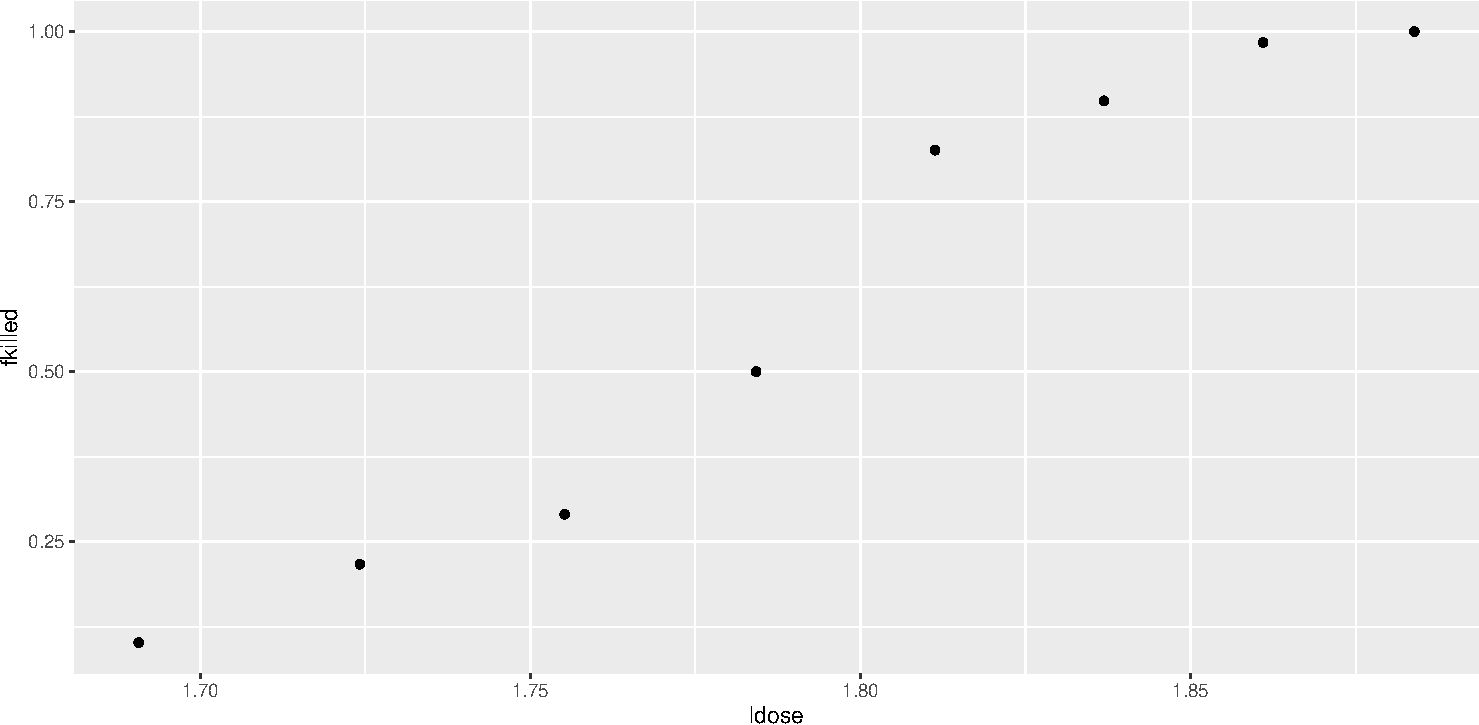
\includegraphics{Module03PresentationWeek1_files/figure-beamer/unnamed-chunk-2-1.pdf}
\end{frame}

\begin{frame}
\textbf{Q}:

\begin{enumerate}
[a.]
\tightlist
\item
  What might be the effect (mathematical function) of the log10-dose on
  the probability of killing a beetle?
\item
  How can this curve be part of a regression model?
\end{enumerate}
\end{frame}

\begin{frame}{How to model a binary response?}
\protect\hypertarget{how-to-model-a-binary-response}{}
In multiple linear regression we have

\begin{enumerate}
\item
  Random component: Distribution of response:
  \(Y_i\sim N(\mu_i,\sigma^2)\), where \(\mu_i\) is \emph{parameter of
  interest} and \(\sigma^2\) is \emph{nuisance}.
\item
  Systematic component: Linear predictor:
  \(\eta_i={\bf x}_i^T \boldsymbol{\beta}\). Here \({\bf x}_i\) is our
  fixed (not random) \(p\)-dimensional column vector of covariates
  (intercept included).
\item
  Link: Connection between the linear predictor and the mean (parameter
  of interest): \(\mu_i=\eta_i\).
\end{enumerate}

\begin{itemize}
\tightlist
\item
  It would not make sense to fit the continuous linear regression to
  \(Y_i\) when \(Y_i=\{0,1\}\) - since \(Y_i\) is not a continuous
  random variable, and \(Y_i\) is not normal.
\item
  So, we need to change 1. We keep 2. And, we make 3. more general.
\end{itemize}
\end{frame}

\begin{frame}
\begin{block}{Binary regression}
\protect\hypertarget{binary-regression}{}
\begin{enumerate}
\tightlist
\item
  \(Y_i \sim \text{bin}(n_i,\pi_i)\).
\end{enumerate}

First look at \(n_i=1\) (i.e.~a Bernoulli distribution).

Our parameter of interest is \(\pi_i\) which is the mean
\(\text{E}(Y_i)=\mu_i=\pi_i\).

\textbf{For a generalized linear model (GLM) we require that the
distribution of the response is an exponential family. We have seen in
M1 that the binomial distribution is an exponential family.}
\end{block}
\end{frame}

\begin{frame}
\begin{block}{Linear Predictor}
\protect\hypertarget{linear-predictor}{}
\(\eta_i={\bf x}_i^T \boldsymbol{\beta}\).
\end{block}
\end{frame}

\begin{frame}
\begin{block}{Link Function}
\protect\hypertarget{link-function}{}
\begin{enumerate}
\setcounter{enumi}{2}
\tightlist
\item
  Relationships between the mean \(\mu_i=\pi_i\) and the linear
  predictor \(\eta_i\):
\end{enumerate}

\[
g(\mu_i)=\eta_i
\]

and the inverse of the link function, called the \emph{response
function}, and denoted by

\[
h(\eta_i)=g^{-1}(\eta_i)=\mu_i
\]

We thus also have to require that the link function is monotone, and we
will soon see that we also need to require that it is twice
differential.
\end{block}
\end{frame}

\begin{frame}
\begin{block}{Response function for binary regression}
\protect\hypertarget{response-function-for-binary-regression}{}
Based on selecting a cumulative distribution function (cdf) as the
response function.

The cdf will always be within {[}0,1{]}, and the cdf is monotone - which
will help us to interpret results.

The most popular response functions are:

\begin{itemize}
\tightlist
\item
  \emph{logistic cdf} (with corresponding \emph{logit} link function)
  referred to as the \emph{logit model},
\item
  \emph{normal cdf} - (with corresponding \emph{probit} link function)
  referred to as the \emph{probit model} ,
\item
  the \emph{extreme minimum-value cdf} (with corresponding
  \emph{complementary log-log} link function) referred to as the
  \emph{complementary log-log model}.
\end{itemize}

In this module we focus on the logit model.
\end{block}
\end{frame}

\begin{frame}
\begin{block}{The logit model aka logistic regression}
\protect\hypertarget{the-logit-model-aka-logistic-regression}{}
In the beetle example we have a simple linear predictor:
\(\eta_i=\beta_0+\beta_1 x_i\) where \(x_i\) is the log10-dose for
beetle \(i\).

Assume that \(\beta_0=\) -60.1 and \(\beta_1=\) 33.9. (These values are
estimates from our data, and we will see later how to find these
estimates using maximum likelihood estimation.)
\end{block}
\end{frame}

\begin{frame}
Below the response function is plotted for \(\eta_i=\)-60.1+33.9\(x_i\).

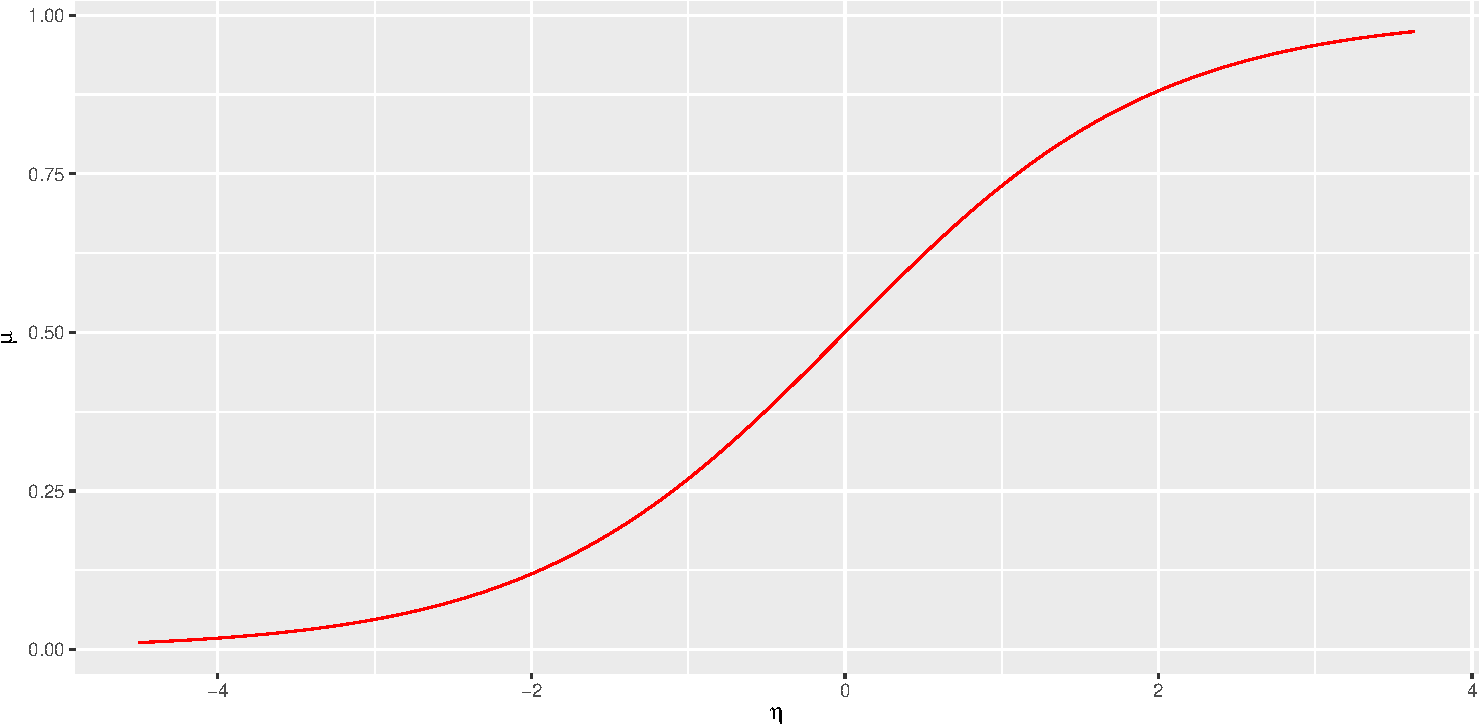
\includegraphics{Module03PresentationWeek1_files/figure-beamer/unnamed-chunk-5-1.pdf}

\textbf{Q}: Explain to your neighbour what is on the x- and y-axis of
this plot. Where are the observed log10-doses in this graph?
\end{frame}

\begin{frame}
\begin{block}{Link and reponse function}
\protect\hypertarget{link-and-reponse-function}{}
The logit model is based on the logistic cdf as the response function,
given as \[ \mu_i=\pi_i=h(\eta_i)=\frac{\exp(\eta_i)}{1+\exp(\eta_i)}\]
or alternatively as the link function (the inverse of the response
function)
\[ g(\mu_i)=h^{-1}(\mu_i)=\ln(\frac{\mu_i}{1-\mu_i})=\ln(\frac{\pi_i}{1-\pi_i})\]

\textbf{Hands-on}: show this for yourself.
\end{block}
\end{frame}

\begin{frame}
\begin{block}{Interpreting the logit model}
\protect\hypertarget{interpreting-the-logit-model}{}
If the value of the linear predictor \(\eta_i\) changes to \(\eta_i+1\)
the probability \(\pi\) increases non-linearly from
\(\frac{\exp(\eta_i)}{1+\exp(\eta_i)}\) to
\(\frac{\exp(\eta_i+1)}{1+\exp(\eta_i+1)}\), as shown in the graph
above.
\end{block}
\end{frame}

\begin{frame}
Before we go further: do you know about the odds? The ratio
\(\frac{P(Y_i=1)}{P(Y_i=0)}=\frac{\pi_i}{1-\pi_1}\) is called the
\emph{odds}. If \(\pi_i=\frac{1}{2}\) then the odds is \(1\), and if
\(\pi_i=\frac{1}{4}\) then the odds is \(\frac{1}{3}\). We may make a
table for probability vs.~odds in R:

\begin{table}
\centering
\begin{tabular}{l|r|r|r|r|r|r|r|r|r}
\hline
pivec & 0.10 & 0.20 & 0.30 & 0.40 & 0.5 & 0.6 & 0.70 & 0.8 & 0.9\\
\hline
odds & 0.11 & 0.25 & 0.43 & 0.67 & 1.0 & 1.5 & 2.33 & 4.0 & 9.0\\
\hline
\end{tabular}
\end{table}
\end{frame}

\begin{frame}
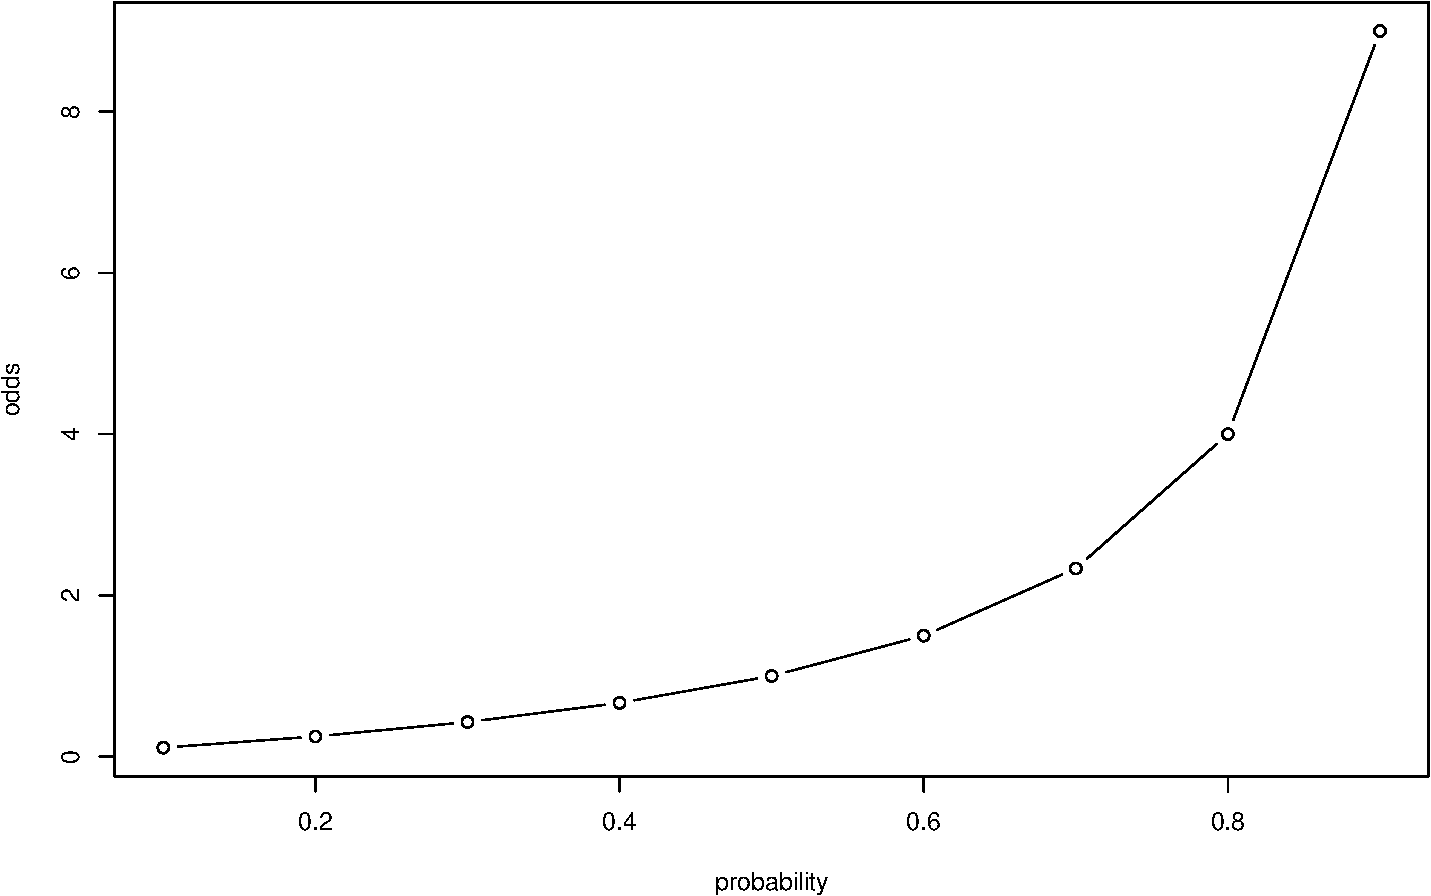
\includegraphics{Module03PresentationWeek1_files/figure-beamer/unnamed-chunk-7-1.pdf}

Odds may be seen to be a better scale than probability to represent
chance, and is used in betting. In addition, odds are unbounded above.
\end{frame}

\begin{frame}
We look at the link function (inverse of the response function). Let us
assume that our linear predictor has \(k\) covariates present

\begin{align*}
\eta_i&= \beta_0+\beta_1 x_{i1}+\beta_2 x_{i2}+\cdots + \beta_k x_{ik}\\
\pi_i&= \frac{\exp(\eta_i)}{1+\exp(\eta_i)}\\
\eta_i&=\ln(\frac{\pi_i}{1-\pi_i})\\
\ln(\frac{\pi_i}{1-\pi_i})&=\beta_0+\beta_1 x_{i1}+\beta_2 x_{i2}+\cdots + \beta_k x_{ik}\\
\frac{\pi_i}{1-\pi_i}=&\frac{P(Y_i=1)}{P(Y_i=0)}=\exp(\beta_0)\cdot \exp(\beta_1 x_{i1})\cdots\exp(\beta_k x_{ik})
\end{align*}

We have a \emph{multiplicative model} for the odds.
\end{frame}

\begin{frame}
\textbf{So, what if we increase \(x_{1i}\) to \(x_{1i}+1\)?}

If the covariate \(x_{1i}\) increases by one unit (while all other
covariates are kept fixed) then the odds is multiplied by
\(\exp(\beta_1)\):

\begin{align*}
\frac{P(Y_i=1\mid x_{i1}+1)}{P(Y_i=0)\mid x_{i1}+1)}&=\exp(\beta_0)\cdot \exp(\beta_1 (x_{i1}+1))\cdots\exp(\beta_k x_{ik})\\
&=\exp(\beta_0)\cdot \exp(\beta_1 x_{i1})\exp(\beta_1)\cdots\exp(\beta_k x_{ik})\\
&=\frac{P(Y_i=1\mid x_{i1})}{P(Y_i=0\mid x_{i1})}\cdot \exp(\beta_1)\\
\end{align*}

This means that if \(x_{i1}\) increases by \(1\) then: if \(\beta_1<0\)
we get a decrease in the odds, if \(\beta_1=0\) no change, and if
\(\beta_1>0\) we have an increase. In the logit model \(\exp(\beta_1)\)
can be easier to interpret than \(\beta_1\).
\end{frame}

\begin{frame}
\begin{block}{To Sum Up}
\protect\hypertarget{to-sum-up}{}
For the linear predictor we interpret effects in the same way as for the
linear model (in Module 2), then we transform this linear effect in
\(\eta\) into a nonlinear effect for
\(\pi=\frac{\exp(\eta)}{1+\exp(\eta)}\), and use the odds to interpret
changes.

\textbf{Q:} If \(x_{i1}\) increases by \(1\) AND\(\beta_1\) is small,
what is the relationship between the change in the odds, the change in
the log odds and the change in the probability?
\end{block}
\end{frame}

\begin{frame}
\begin{block}{Infant respiratory disease: interpretating parameter
estimates}
\protect\hypertarget{infant-respiratory-disease-interpretating-parameter-estimates}{}
This example is taken from Faraway (2006): ``Extending the linear model
with R''

We select a sample of newborn babies (girls and boys) where the parents
had decided on the method of feeding (bottle, breast, breast with some
supplement), and then monitored the babies during their first year to
see if they developed infant respiratory disease (the event we want to
model).

We fit a logistic regression to the data, and focus on the parameter
estimates.
\end{block}
\end{frame}

\begin{frame}[fragile]
\begin{Shaded}
\begin{Highlighting}[]
\FunctionTok{library}\NormalTok{(faraway)}
\FunctionTok{data}\NormalTok{(babyfood)}
\CommentTok{\# babyfood}
\FunctionTok{xtabs}\NormalTok{(disease}\SpecialCharTok{/}\NormalTok{(disease}\SpecialCharTok{+}\NormalTok{nondisease)}\SpecialCharTok{\textasciitilde{}}\NormalTok{sex}\SpecialCharTok{+}\NormalTok{food,babyfood)}
\end{Highlighting}
\end{Shaded}

\begin{verbatim}
##       food
## sex        Bottle     Breast      Suppl
##   Boy  0.16812227 0.09514170 0.12925170
##   Girl 0.12500000 0.06681034 0.12598425
\end{verbatim}
\end{frame}

\begin{frame}
\begin{tabular}{l|r|r|r|r}
\hline
  & Estimate & Std. Error & z value & Pr(>|z|)\\
\hline
(Intercept) & -1.61 & 0.11 & -14.35 & 0.00\\
\hline
sexGirl & -0.31 & 0.14 & -2.22 & 0.03\\
\hline
foodBreast & -0.67 & 0.15 & -4.37 & 0.00\\
\hline
foodSuppl & -0.17 & 0.21 & -0.84 & 0.40\\
\hline
\end{tabular}
\end{frame}

\begin{frame}[fragile]
\begin{block}{Questions}
\protect\hypertarget{questions}{}
Observe that the two factors by default is coded with dummy variable
coding, and that \texttt{sexBoy} is the reference category for sex and
\texttt{foodBottle} the reference category for feeding method.

1: Explain how to interpret the \texttt{Estimate} for \texttt{sexGirl},
\texttt{foodBreast} and \texttt{foodSuppl}.

2: What are the 6 values given by the call to \texttt{predict}? What is
the least favourable combination of sex and method of feeding? And the
most favourable?

\begin{Shaded}
\begin{Highlighting}[]
\FunctionTok{print}\NormalTok{(}\FunctionTok{predict}\NormalTok{(fit,}\AttributeTok{type=}\StringTok{"response"}\NormalTok{), }\AttributeTok{digits=}\DecValTok{2}\NormalTok{) }\CommentTok{\#gives predicted probabilites}
\end{Highlighting}
\end{Shaded}

\begin{verbatim}
##     1     2     3     4     5     6 
## 0.166 0.144 0.093 0.127 0.109 0.069
\end{verbatim}
\end{block}
\end{frame}

\begin{frame}
\begin{block}{More response function plots for the logit model}
\protect\hypertarget{more-response-function-plots-for-the-logit-model}{}
The response function as a function of the covariate \(x\) and not of
\(\eta\). Solid lines: \(\beta_0=0\) and \(\beta_1\) is \(0.8\) (blue),
\(1\) (red) and \(2\) (orange), and dashed lines with \(\beta_0=1\).

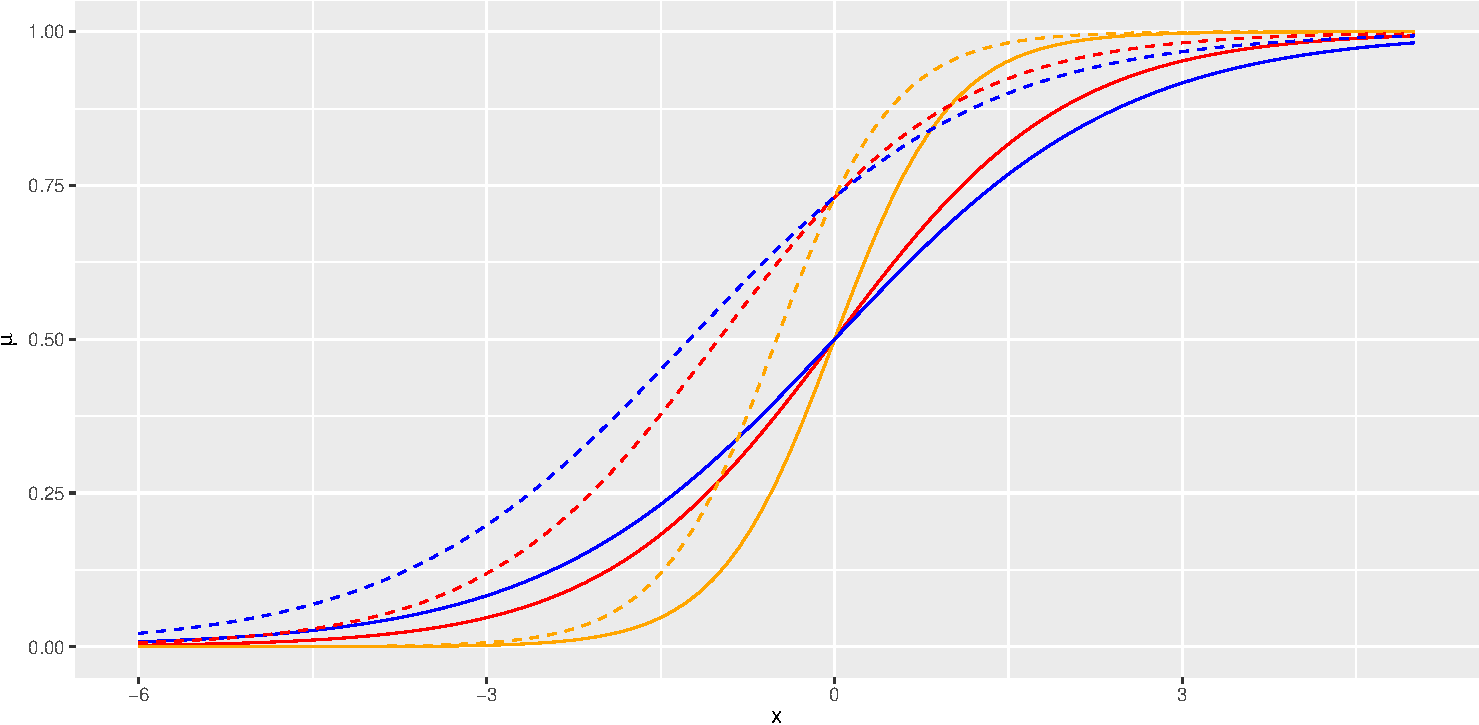
\includegraphics{Module03PresentationWeek1_files/figure-beamer/unnamed-chunk-10-1.pdf}
\end{block}
\end{frame}

\begin{frame}{Grouped vs.~individual data}
\protect\hypertarget{grouped-vs.-individual-data}{}
So far we have only mentioned individual data.

However, in both the examples we have looked at some covariate vectors
are \emph{identical} (rows in the design matrix are identical). We call
these unique combinations of covariates \emph{covariate patterns}, and
say we have \emph{grouped} data.

\begin{table}
\centering
\begin{tabular}{r|r|l|l}
\hline
disease & nondisease & sex & food\\
\hline
77 & 381 & Boy & Bottle\\
\hline
19 & 128 & Boy & Suppl\\
\hline
47 & 447 & Boy & Breast\\
\hline
48 & 336 & Girl & Bottle\\
\hline
16 & 111 & Girl & Suppl\\
\hline
31 & 433 & Girl & Breast\\
\hline
\end{tabular}
\end{table}
\end{frame}

\begin{frame}[fragile]
Here we have 6 groups of covariate patterns. The first group has
covariates \texttt{Boy} and \texttt{Bottle}, there are 77+381= 458
babies with this combination and 77 of these got the disease.

We prefer to group data if possible. Grouping is good because then data
can be kept in a condensed form, it will speed up computations and makes
model diagnosis easier (than for individual data).
\end{frame}

\begin{frame}
For the grouped data we still have a binomial distribution, and possible
generalization is to let

\begin{itemize}
\tightlist
\item
  \(n_j\bar{Y_j}\) be the number of successes in group \(j\),
\item
  which means that \(\bar{Y_j}=\frac{1}{n_j}\sum Y_i\) where the sum is
  over all \(i\) in group \(j\).
\end{itemize}

Further \[ n_j\bar{Y_j} \sim \text{bin}(n_j,\pi_j)\] such that
\(\text{E}(n_j\bar{Y_j})=n_j \pi_j\) and
\(\text{Var}(n_j\bar{Y_j})=n_j \pi_j(1-\pi_j)\), and
\(\text{E}(\bar{Y_j})=\pi_j\) and
\(\text{Var}(\bar{Y_j})=\frac{1}{n_j} \pi_j(1-\pi_j)\)

We then keep the linear predictor, and the link function is still
\(\eta_j=\ln(\frac{\pi_j}{1-\pi_j})\). That is, we do not model the mean
\(n_j \pi_j\) but \(\pi_j\) directly.
\end{frame}

\begin{frame}{Likelihood and derivations thereof}
\protect\hypertarget{likelihood-and-derivations-thereof}{}
Our parameter of interest is the vector \(\boldsymbol{\beta}\) of
regression coefficients, and we have no nuicance parameters (because the
variance is related directly to the \(\pi_j\) and \(n_j\) is known).

We would like to estimate \(\boldsymbol{\beta}\) from maximizing the
likelihood, but we will soon see that we have no closed form solution.
First we look at the likelihood, the log-likelihood and first and second
derivatives thereof.

For simplicity we do the derivations for the case where \(n_i=1\), but
then include the results for the case where we have \(G\) covariate
patterns with \(n_j\) observations of each pattern.
\end{frame}

\begin{frame}
\begin{block}{Assumptions}
\protect\hypertarget{assumptions}{}
\begin{enumerate}
\tightlist
\item
  \(Y_i \sim \text{bin}(n_i=1,\pi_i)\), and
  \(\text{E}(Y_i)=\mu_i=\pi_i\), and \(\text{Var}(Y_i)=\pi_i(1-\pi_i)\).
\item
  Linear predictor: \(\eta_i={\bf x}_i^T \boldsymbol{\beta}\).
\item
  Logit link \[\eta_i=\ln(\frac{\pi_i}{1-\pi_i})=g(\mu_i)\] and (inverse
  thereof) logistic response function
  \[\mu_i=\pi_i=\frac{\exp(\eta_i)}{1+\exp(\eta_i)}=h(\eta_i)\]
\end{enumerate}

We will also need:
\[(1-\pi_i)=1-\frac{\exp(\eta_i)}{1+\exp(\eta_i)}=\frac{1+\exp(\eta_i)-\exp(\eta_i)}{1+\exp(\eta_i)}=\frac{1}{1+\exp(\eta_i)}.\]
\end{block}
\end{frame}

\begin{frame}
\begin{block}{Likelihood \(L(\boldsymbol{\beta})\)}
\protect\hypertarget{likelihood-lboldsymbolbeta}{}
We assume that pairs of covariates and response are measured
independently of each other: \(({\bf x}_i,Y_i)\), and \(Y_i\) follows
the distribution specified above, and \({\bf x}_i\) is fixed.

\[L(\boldsymbol{\beta})=\prod_{i=1}^n L_i(\boldsymbol{\beta})=\prod_{i=1}^n f(y_i; \boldsymbol{\beta})=\prod_{i=1}^n\pi_i^{y_i}(1-\pi_i)^{1-y_i}\]
\end{block}
\end{frame}

\begin{frame}
\begin{block}{Loglikelihood \(l(\boldsymbol{\beta})\)}
\protect\hypertarget{loglikelihood-lboldsymbolbeta}{}
\begin{align}
l(\boldsymbol{\beta})&=\ln L(\boldsymbol{\beta})=\sum_{i=1}^n \ln L_i(\boldsymbol{\beta})=\sum_{i=1}^n l_i(\boldsymbol{\beta})\\
&=\sum_{i=1}^n[y_i \ln \pi_i+(1-y_i) \ln(1-\pi_i)]\\
&=\sum_{i=1}^n[y_i \ln (\frac{\pi_i}{1-\pi_i})+\ln(1-\pi_i)]
\end{align}

Observe that the log-likelihood is a sum of invidual contributions for
each observation pair \(i\).
\end{block}
\end{frame}

\begin{frame}
The log-likelihood is now expressed as a function of \(\pi_i\), but we
want to make this a function of \(\boldsymbol{\beta}\) and the
connection between \(\pi_i\) and \(\boldsymbol{\beta}\) goes through
\(\eta_i\). We have that \(\pi=\frac{\exp(\eta_i)}{1+\exp(\eta_i)}\) and
in our log-likelihood we need

\[(1-\pi_i)=\frac{1}{1+\exp(\eta_i)}=\frac{1+\exp(\eta_i)-\exp(\eta_i)}{1+\exp(\eta_i)}=\frac{1}{1+\exp(\eta_i)}\]
and

\[\ln(\frac{\pi_i}{1-\pi_1})=\eta_i\] (the last is our logit link
function).
\end{frame}

\begin{frame}
Then we get:

\[l(\boldsymbol{\beta})=\sum_{i=1}^n[y_i \eta_i + \ln (\frac{1}{1+\exp(\eta_i)})]=\sum_{i=1}^n[y_i \eta_i - \ln (1+\exp(\eta_i))]\]
which is now our function of \(\eta_i\).

Finally, since \(\eta_i={\bf x}_i^T \boldsymbol{\beta}\),
\[l(\boldsymbol{\beta})=\sum_{i=1}^n[y_i {\bf x}_i^T \boldsymbol{\beta} - \ln (1+\exp({\bf x}_i^T \boldsymbol{\beta}))].\]
\end{frame}

\begin{frame}
\textbf{Q}: What does the graph of \(l\) look like as a function of
\(\boldsymbol{\beta}\)?

If we look at the beetle example we only have one covariate (in addition
to the intercept) - so this means that we have
\(\boldsymbol{\beta}=(\beta_0,\beta_1)\). Plotting the log-likelihood
(for the beetle data set) will be one of the tasks for the interactive
lecture.

\textbf{But, next we take partial derivatives, and then we will (instead
of using this formula) look at
\(l_i(\boldsymbol{\beta})=l_i(\eta_i(\boldsymbol{\beta}))\) and use the
chain rule.}
\end{frame}

\begin{frame}
\begin{block}{Score function \(s(\boldsymbol{\beta})\)}
\protect\hypertarget{score-function-sboldsymbolbeta}{}
The score function is a \(p\times 1\) vector, \(s(\boldsymbol{\beta})\),
with the partial derivatives of the log-likelihood with respect to the
\(p\) elements of the \(\boldsymbol{\beta}\) vector.

Solving \(s(\boldsymbol{\beta})=0\) wil give us our MLEs
\end{block}
\end{frame}

\begin{frame}
We will need the following:

Chain rule: \(\frac{d f(u(x))}{du}=\frac{df}{du}\cdot \frac{du}{dx}\),

Product rule: \((u\cdot v)'=u'\cdot v+u\cdot v'\),

Fraction rule: \((\frac{u}{v})'=\frac{u' \cdot v - u\cdot v'}{v^2}\),

\(\frac{d \ln(x)}{dx}=\frac{1}{x}\), \(\frac{d\exp(x)}{dx}=\exp(x)\) and
\(\frac{d(\frac{1}{x})}{dx}=-\frac{1}{x^2}\).

Partial derivatives of scalar wrt a vector
\(\frac{\partial{\bf a}^T{\bf b}}{\partial {\bf b}}={\bf a}\)

and later we will also need
\(\frac{\partial{\bf a}^T{\bf b}}{\partial {\bf b}^T}=(\frac{\partial{\bf a}^T{\bf b}}{\partial {\bf b}})^T={\bf a}^T.\)
\end{frame}

\begin{frame}
Here we go:
\[s(\boldsymbol{\beta})=\frac{\partial l(\boldsymbol{\beta})}{\partial \boldsymbol{\beta}}=
\sum_{i=1}^n \frac{\partial l_i(\boldsymbol{\beta})}{\partial \boldsymbol{\beta}}=
\sum_{i=1}^n s_i(\boldsymbol{\beta})\]

Again, observe that the score function is a sum of individual
contributions for each observation pair \(i\).
\end{frame}

\begin{frame}
We will use the chain rule to calculate \(s_i(\boldsymbol{\beta})\).

\[s_i(\boldsymbol{\beta})=\frac{\partial l_i(\boldsymbol{\beta})}{\partial \boldsymbol{\beta}}=\frac{\partial l_i(\boldsymbol{\beta})}{\partial \eta_i}\cdot \frac{\partial \eta_i}{\partial \boldsymbol{\beta}}=\frac{\partial [y_i\eta_i-\ln(1+{\exp(\eta_i)})]}{\partial \eta_i}\cdot \frac{\partial [{\bf x}_i^T\boldsymbol{\beta} ]}{\partial \boldsymbol{\beta}}\]

\[s_i(\boldsymbol{\beta})=(y_i-\frac{\exp(\eta_i)}{1+\exp(\eta_i)})\cdot {\bf x}_i=(y_i-\pi_i) {\bf x}_i \]
\end{frame}

\begin{frame}
The score function is given as:

\[s(\boldsymbol{\beta})=\sum_{i=1}^n s_i(\boldsymbol{\beta})=\sum_{i=1}^n {\bf x}_i (y_i-\pi_i)=\sum_{i=1}^n {\bf x}_i (y_i-\frac{\exp({\bf x}_i^T\boldsymbol{\beta})}{1+\exp({\bf x}_i^T\boldsymbol{\beta})})\]

To find the maximum likelihood estimate \(\hat{\boldsymbol{\beta}}\) we
solve the set of \(p\) non-linear equations:
\[s(\hat{\boldsymbol{\beta}})=0\]

Next week we will see how we can do that using the Newton-Raphson or
Fisher Scoring iterative methods, but first we will work on finding the
mean and covariance matrix of the score vector - and the derivatives of
the score vector (the Hessian, which is minus the observed Fisher
matrix).
\end{frame}

\begin{frame}
\textbf{Remark}: in Module 5 we will see that the general formula for
GLMs is: \[s(\boldsymbol{\beta})=\sum_{i=1}^n
[\frac{y_i-\mu_i}{\text{Var}(Y_i)}{\bf x}_i \frac{\partial \mu_i}{\partial \eta_i}]=\sum_{i=1}^n
[\frac{y_i-\mu_i}{\text{Var}(Y_i)}{\bf x}_i h'(\eta_i)]={\bf X}^T {\bf D} \Sigma^{-1} ({\bf y} -\mu)\]
where \({\bf X}\) is the \(n\times p\) design matrix,
\({\bf D}=\text{diag}(h'(\eta_1),h'(\eta_2),\ldots,h'(\eta_n))\) is a
diagonal matrix with the derivatives of the response function evaluated
at each observation. Further,
\(\Sigma=\text{diag}(\text{Var}(Y_1),\text{Var}(Y_2),\ldots,\text{Var}(Y_n))\)
is a diagonal matrix with the variance for each response, and
\({\bf y}\) is the observed \(n\times 1\) vector of responses and
\(\mu\) is the \(n\times 1\) vector of individual expectations
\(\mu_i=\text{E}(Y_i)=h(\eta_i)\).
\end{frame}

\begin{frame}
\end{frame}

\end{document}
